\chapter{Boosted VHbb Analysis}\label{chap:vhbb_boosted}

The Higgs boson, discovered at the LHC in 2012 \cite{HIGG-2012-27,CMS-HIG-12-028}, is predicted by the standard model to decay primarily to two \bquarks, with a branching factor of $0.582 \pm 0.007$ \cite{deFlorian:2016spz}. 
Observation of this decay mode was reported by \ATLAS \cite{HIGG-2018-04} and \CMS \cite{CMS-HIG-18-016} in 2018.
Whilst the dominant Higgs production mechanism at the LHC is gluon-gluon fusion as outlined in \cref{sec:higgs_pheno}, this mechanism has an overwhelming QCD multijet background and so overall sensitivity to the Higgs is low.
The \hbb observation therefore searched for Higgs bosons produced in association with a vector boson (\Wboson or \Zboson).
This production mechanism results in leptonic final states from the decay of the vector boson, allowing for leptonic triggering, whilst at the same time significantly reducing the multi-jet background.

A closely related analysis \cite{HIGG-2018-52} measured the associated production of a Higgs boson decaying to \bquarks in events where the vector and Higgs bosons are highly boosted.
The analysis is outlined in \cref{sec:vhbb_overview}.
Modelling studies are listed in \cref{sec:vhbb_modelling}, and the results of the analysis are presented in \cref{sec:vhbb_results}.
The author contributed to various signal and background modelling studies, fit studies, and to the diboson unblinding effort.
This analysis has been published in \rcite{HIGG-2018-52}.
Figures and tables from \rcite{HIGG-2018-52} are reproduced here.
\todo{cite internal note?}

\begin{comment}
  In particular, the observation of the decay of the
Higgs boson into $b$-quark pairs provided direct evidence for the
Yukawa coupling of the Higgs boson to down-type
quarks~\cite{HIGG-2018-04,CMS-HIG-18-016}.  Finally, a combination
of \SI{13}{\TeV} results searching for the Higgs boson produced in
association with a leptonically decaying \Wboson or \Zboson boson established
the observation of this production process~\cite{HIGG-2018-04}.
%These analyses were
%aiming at vector bosons with transverse momentum in the
%approximate range [100--300]~\GeV.
A first cross-section measurement as a
function of the vector-boson transverse momentum was also carried out
by the ATLAS Collaboration~\cite{HIGG-2018-50}.

%In particular, the observation of the decay of the
%Higgs boson to $b$-quark pairs when produced in association with a leptonically decaying $W$ or $Z$ boson provided direct
%evidence for the Yukawa coupling of the Higgs boson to down-type quarks
%and also established the observation of this production
%process

The previous ATLAS analyses~\cite{HIGG-2018-04,HIGG-2018-50} in this
channel were mainly sensitive to vector bosons with transverse
momentum ($\pt$) in the range of approximately 100--\SI{300}{\GeV}. These
analyses considered a pair of jets with radius parameter of $R= 0.4$,
referred to as small-radius (\smallR) jets, to reconstruct the Higgs
boson. For higher Higgs boson transverse momenta, the decay products
can become close enough that they cannot be reconstructed with
two \smallR\ jets.  To explore this `boosted' regime, the Higgs boson
is reconstructed as a single \largeR\ jet with
$R=1.0$~\cite{Butterworth:2008iy}.
%that is subsequently
%decomposed using jet substructure
%techniques.
This high-\pt\ regime is particularly interesting due to
its sensitivity to physics beyond the Standard
Model~\cite{Mimasu:2015nqa}.
\end{comment}


\section{Analysis Overview}\label{sec:vhbb_overview}

The boosted \VHbb analysis is focused on the high transverse momentum regime.\todo{why interesting?}
As such, the reconstructed vector boson is required to have $\ptv > \SI{250}{\GeV}$.
Events are split into two \ptv bins with the first bin covering $\SI{250}{\GeV} < \ptv < \SI{400}{\GeV}$ and the second covering $\ptv > \SI{400}{\GeV}$.
The full \runtwo dataset at \come{13} is used for a total integrated luminosity of \intlumi.

On top of the binning in \ptv, the events are further categorised into 0-, 1- and 2-lepton channels depending on the number of selected charged leptons (electrons and muons) are present in the reconstructed final state.
The 0-lepton channel targets the $\Zboson \higgs \rightarrow \nu\nu \bbbar$ process, the 1-lepton channel targets $\Wboson \higgs \rightarrow \ell\nu \bbbar$, while the 2-lepton channel targets $\Zboson \higgs \rightarrow \ell\ell \bbbar$, where $\ell$ is an electron or muon and $\nu$ is a neutrino.
In all channels, events are required to have exactly two \btagged $R=0.2$ trackjets (see \cref{sec:jet_reco}), which are used to reconstruct the Higgs boson candidate.
At least one of the \btagged jets is required to have \pT greater than 45 GeV.
Events are further split into 2-jet or 3-jet categories depending on whether additional untagged jets are present. 

%  The \hbb\ decay is reconstructed using a
% jet with transverse momentum $p_{\mathrm{T}} > \SI{250}{\GeV}$, found with
% the \antikt $R = 1.0$ jet algorithm, and groomed to remove soft
% and wide-angle radiation and to mitigate contributions from the
% underlying event and additional proton-proton collisions. Higgs
% bosons are identified using \btagged $R = 0.2$ track-jets matched
% to the groomed \largeR\ calorimeter jets. 

\subsection{Analsysis Selections}

%
\begin{sidewaystable}[p]
    \footnotesize\centering
    \setlength{\extrarowheight}{2pt}
    \begin{tabular}{l | c|c|c|c|c|c}
      \toprule\hline
      Selection & \multicolumn{2}{c|}{0 lepton channel} & \multicolumn{2}{c|}{1 lepton channel} & \multicolumn{2}{c}{2 leptons channel} \\
      & \multicolumn{2}{c|}{} & $e$ sub-channel & $\mu$ sub-channel & $e$ sub-channel & $\mu$ sub-channel \\
      \hline
      Trigger & \multicolumn{2}{c|}{ \met } &  Single electron & \met & Single electron & \met \\
      \hline
      Leptons & \multicolumn{2}{c|}{0 \VHloose\ leptons} & \multicolumn{2}{c|}{1 \WHsignal\ lepton} & \multicolumn{2}{c}{2 \VHloose\ leptons among which} \\
      & \multicolumn{2}{c|}{ } &  $\pt>27$~GeV & $\pt>25$~GeV & \multicolumn{2}{c}{ $\geq$ 1 \WHsignal\ lepton, $\pt>27$~GeV } \\
      & \multicolumn{2}{c|}{ } &  \multicolumn{2}{c|}{no second \VHloose\ lepton}  & \multicolumn{2}{c}{both leptons of the same flavour} \\
      & \multicolumn{2}{c|}{ } &  \multicolumn{2}{c|}{ }  & - & opposite sign muons  \\
      
      \hline
      \met & \multicolumn{2}{c|}{ $> 250$ GeV} & $> 50$ GeV & -  & \multicolumn{2}{c}{-} \\
      \hline
      \pTV & \multicolumn{6}{c}{$\pTV > 250$ GeV } \\
      \hline
      %Jets & \multicolumn{6}{c}{ at least one large-\textit{R} jet} \\
      %\hline
      %Large-R jet \pt & \multicolumn{6}{c}{ > 250 GeV} \\
      \LargeR jets & \multicolumn{6}{c}{ at least one large-\textit{R} jet, $\pt> 250$ GeV, $|\eta| < 2.0$} \\
      \hline
      Track-jets & \multicolumn{6}{c}{at least two track-jets, $\pt > 10$ GeV,  $|\eta| < 2.5$, matched to the leading large-\textit{R} jet} \\
      \hline
      $b$-tagged jets & \multicolumn{6}{c}{leading two track-jets matched to the leading large-\textit{R} must be $b$-tagged (MV2c10, 70\%)} \\
      \hline
      \mJ      & \multicolumn{6}{c}{$> 50$ GeV} \\
      \hline
      $\min[\Delta \phi$(\vecmet, \smallR\ jets)] & \multicolumn{2}{c|}{ $> 30^{\circ}$} & \multicolumn{4}{c}{-} \\
      \hline
      $\Delta \phi$(\vecmet, $H_{\text{cand}}$) & \multicolumn{2}{c|}{ $> 120^{\circ}$} & \multicolumn{4}{c}{-} \\
      \hline
      $\Delta \phi$ (\vecmet, \vecmpt) & \multicolumn{2}{c|}{ $< 90^{\circ}$} & \multicolumn{4}{c}{-} \\
      \hline
      $\Delta y (V, H_{\text{cand}})$ & \multicolumn{2}{c|}{-} & \multicolumn{4}{c}{$|\Delta y (V, H_{\text{cand}})| < 1.4$} \\
      \hline
      \mll & \multicolumn{4}{c|}{-} & \multicolumn{2}{c}{ 66 GeV $< \mll < 116$ GeV} \\
      \hline
      Lepton \pT imbalance & \multicolumn{4}{c|}{-} & \multicolumn{2}{c}{$(\pT^{\ell_{1}} - \pT^{\ell_{2}} ) / \pTZ < 0.8$} \\
   %   \hline
  %    Lepton flavour & \multicolumn{4}{c|}{-} & \multicolumn{2}{c}{two leptons of the same flavour} \\
   %   \hline
    %  Lepton charge & \multicolumn{4}{c|}{-} & &opposite \\
    %  			 & \multicolumn{4}{c|}{-} & & sign muons \\
  
  %    \pTV regions & \multicolumn{6}{c}{250 GeV < \pTV < 400 GeV  and \pTV > 400 GeV } \\
  %    \hline
  %    \hline
  %    \multirow{2}{*}{Signal regions} & \multicolumn{4}{c|}{ 0 add. small-R jets, > 1 add. small-R jets } & \multicolumn{2}{c}{\multirow{2}{*}{-}} \\
  %    \cline{2-5}
  %    & \multicolumn{4}{c|}{ 0 add. \btagged track-jets} & \multicolumn{2}{c}{}\\
  %    \hline
  %    \hline
  %    Control regions &  \multicolumn{4}{c|}{> 1 add. \btagged track-jets} &  \multicolumn{2}{c}{ - } \\
      \hline\bottomrule
    \end{tabular}
    \caption{
        Event selection requirements for the boosted $VH$, \Hbb analysis channels and sub-channels \cite{HIGG-2018-52}.
        Various channel dependent selections are used to maximise the signal efficiency and reduce the number of background events in each analysis region.
    }
    \label{tab:vhbb_selection}
\end{sidewaystable}
  
%

\subsection{Signal and Control Regions}

In the 0- and 1-lepton channels, the analysis is split into signal and control regions.
The signal region (SR) should contain the events with Higgs candidates, while the control region (CR) is pure in \ttbar events and hence used to constrain the normalisation of the \ttbar background.

To leading order, there are no additional $b$-jets in the event other than the two coming from the reconstructed Higgs candidate, which are inside the \largeR jet.
For this reason, there is a signal region veto (i.e. events are not accepted into the signal region) for events with additional \btagged jets in the event.
Events with additional \btagged jets outside the \largeR jet are included in the control region.
In this case, the Higgs candidate (the \largeR jet containing two \btagged trackjets) is likely to be built from the boosted hadronic decay of a top quark (i.e. $t \rightarrow Wb$).
An additional \btagged jet from the other top quark is likely to be present in the event.
, which is highly pure in \ttbar events.


  
\begin{comment}

Lifted from paper intro:

Since the discovery of the Higgs boson
($H$)~\cite{Englert:1964et,Higgs:1964ia,Higgs:1964pj,Guralnik:1964eu}
with a mass of around \SI{125}{\GeV}\cite{HIGG-2014-14} by the ATLAS
%with a mass of around 125~\GeV~\cite{Tanabashi:2018oca} by the ATLAS
and CMS Collaborations~\cite{HIGG-2012-27,CMS-HIG-12-028} in 2012,
the analysis of proton--proton ($pp$) collision data at centre-of-mass
energies of \SI{7}{TeV}, \SI{8}{TeV} and \SI{13}{\TeV} delivered by the Large Hadron
Collider (LHC)~\cite{Evans:2008zzb} has led to precise
measurements of the main production cross-sections and decay rates of
the Higgs boson, as well as measurements of its mass and its spin and
parity properties. 

%an expected branching fraction of approximately 58\% for a mass of
%$\mh=125$~\GeV\ was discovered in 2018 when produced in association
%with a $W$ or $Z$ boson ($VH$) using data collected at Run~2 in 2015,
%2016 and 2017, and at Run~1
%precise measurement of its
%mass (of approximately 125\,\GeV), its  Since then, the analysis of data
%collected has led to the observation of many of the production modes
%and decay channels predicted by the Standard Model (SM).
%As well as probing the dominant decay of
%the Higgs boson, this measurement allows the overall Higgs boson decay
%width~\cite{Lafaye:2009vr,Heinemeyer:2013tqa} to be constrained and
%provides the best sensitivity to the $ZH$ and $WH$ production modes,
%which are (for instance) important elsements in the interpretation of
%Higgs boson measurements in effective field
%theories~\cite{Ellis:2014dva}.



%An
%interesting regime where additional corrections to the high invariant
%mass differential cross-section are expected in the presence of new
%physics beyond SM~\cite{Mimasu:2015nqa}. There are several advantages
%and challenges in the boosted regime. Even though this region
%corresponds to only a small fraction of the total $VH$ cross section
%(about 5\% for $\pT>200$ \GeV), the larger mass of the $VH$ system
%causes it to be central improving the detector signal acceptance and
%large backgrounds with intrinsic scales close to the Higgs mass like
%top-antitop production are largely reduced due to the constrain of
%producing a high-\pt\ $b\bar{b}$ system and a compensating $W/Z$
%boson, without there also being significant additional jet
%activity~\cite{Butterworth:2008iy}. The main challenge is the
%reconstruction of the Higgs boson candidate, since at high transverse
%momenta, the decay products start to merge and they need to be
%reconstructed as a single jet decomposed using jet substructure
%techniques (see Figure~\ref{fig:FeynmanDiagrams}). This analysis has a
%non trivial overlap with the analyses described
%in~\cite{HIGG-2018-04,HIGG-2018-50}, which make use of regular small
%radius calorimeter jets to reconstruct the Higgs boson candidate, and
%has therefore a signal acceptance decreasing significantly with
%increasing vector boson transverse momentum. The overlap in a region
%between approximately 250~\GeV\ and 600~\GeV\ is of the order of 40\%
%and decreases thereafter.

This Letter presents a measurement of cross-sections for the
associated production of a high transverse momentum Higgs boson that
decays into a \bbbar pair with a leptonically decaying $W$ or $Z$
boson. The analysis uses \pp\ collision data recorded between 2015 and
2018 by the ATLAS detector~\cite{PERF-2007-01} during Run~2 at the
LHC. This dataset corresponds to an integrated luminosity
of \intlumi. Events are selected in 0-, 1- and 2-lepton channels,
based on the number of reconstructed charged leptons, $\ell$
(electrons or muons), in the final state to explore the $ZH \to \nu\nu
b\bar{b}$, $WH \to \ell \nu b \bar{b}$ and $ZH \to \ell\ell b\bar{b}$
signatures, respectively. The Higgs boson is reconstructed as a
single \largeR\ jet and the $b$-quarks from its decay as a pair of
jets, reconstructed with a \pt-dependent radius parameter, associated
with the \largeR\ jet and identified as containing a $b$-hadron.

The analysis using \smallR\ jets and focusing on slightly lower Higgs
boson transverse momentum regions was recently updated with the complete Run~2
dataset~\cite{HIGG-2018-51}.
%In the following, $V$ refers to either
%a $W$ or $Z$ boson. For \ptv\ $>$ 250~\GeV\ and up-to
%approximately \ptv\ $<$ 600~\GeV\,
The \largeR\ jet analysis
significantly overlaps with the \smallR\ jets analysis. The two
results can therefore not be straightforwardly combined.


%Therefore, the results from the two
%analyses cannot be straightforwardly combined.


%The candidate
%Higgs-jet is reconstructed using a
%`trimmed’ \antikt~\cite{Cacciari:2008gp} \largeR\
%jet~\cite{PERF-2012-02, Krohn:2009th}, to which two variable-radius
%(VR) track-jets tagged as $b$-jets~\cite{ATL-PHYS-PUB-2014-013,
%PERF-2017-04} are associated.

%(see sketch in
%Figure~\ref{fig:FeynmanDiagrams}).
%using a
%multivariate algorithm based on the tracks impact parameters and the
%reconstruction of secondary vertices, are associated.

%to determine
%associated with the \largeR jet are \btagged, i.e.\ if they contain
%$b$-hadron decay products.

%The approach to tagging presented in this
%Letter is built upon a foundation of studies from LHC runs at
%$\sqrt{s} = 7$ and $8$~\TeV, including extensive studies of jet
%reconstruction and grooming algorithms and detailed investigations of track-jet%-based
%$b$-tagging in boosted topologies~\cite{ATL-PHYS-PUB-2014-013, PERF-2017-04}.
%The \HiggsJet\ mass candidate in the different signal
%regions are used as the discriminant variable and are combined using a
%binned maximum-likelihood fit, referred to as the global likelihood
%fit, which allows the signal yield and the background normalisations
%to be extracted.

The dominant background processes after the event selection correspond
to the production of \vjets, where $V$ refers to either a $W$ or $Z$
boson, \ttbar, single-top and dibosons.  The signal is extracted from
a combined profile likelihood fit to the \largeR jet mass, using
several signal and control regions. The yield of diboson production
$VZ$ with $Z \rightarrow b\bar{b}$ is also measured using the same fit
and provides a validation of the analysis. The cross-section
measurements are performed within the simplified template
cross-section (STXS) framework~\cite{deFlorian:2016spz,
Badger:2016bpw}. These measurements are then used to constrain
anomalous couplings in a Standard Model effective field theory
(SMEFT)~\cite{Contino:2013kra}.

%The
%STXS measurements are designed to proceed in stages of increasing
%granularity with more recorded data.
%In ‘stage 0’, cross-sections are
%measured separately for the four main production modes in a fiducial
%Higgs boson rapidity region $|y_H|< 2.5$ and in ‘stage 1’, these
%regions are split into 31 subregions according to the transverse
%momentum of the weak gauge boson $V$ for $VH$, $V\rightarrow$ leptons
%production. Stage-1 STXS were measured recently for $VH, H\rightarrow
%b\bar{b}$ with 80 \ifb of 13 TeV ATLAS data in the following bins:
%$\ptv<75~\GeV$, $75<\ptv<150~\GeV$ and $\ptv>250~\GeV$, with results in
%agreement with SM predictions~\cite{HIGG-2018-50}. In this letter
%‘stage 1’ results are presented in two kinematic fiducial volumes:
%$250<\ptv>450~\GeV$ and $\ptv>450~\GeV$.

\end{comment}


\section{MC Samples}

\begin{table}[tb!]
    \begin{center}{\fontsize{7}{7.9}\selectfont
    \begin{tabular}{llllll} 
      \toprule
    Process & ME generator & ME PDF &PS and & UE model & Cross-section \hspace{2.5cm}\\
    & & & Hadronisation & tune & order\\ 
    \toprule
    \multicolumn{6}{l}{Signal ($m_H = 125$~GeV and $b\bar{b}$ branching fraction set to 58\%)} \\
    \midrule
     $qq\to WH\to\ell\nu b\bar{b}$  &\textsc{Powheg-Box v2}~\cite{Alioli:2010xd} +&
    NNPDF3.0NLO$^{(\star)}$~\cite{Ball:2014uwa} &\PYTHIAV{8.212}~\cite{Sjostrand:2014zea} & AZNLO~\cite{Aad:2014xaa} & NNLO(QCD)+  \\
            &   \textsc{GoSam}~\cite{Cullen:2011ac} + \textsc{MiNLO}~\cite{Hamilton:2012np,Luisoni:2013kna}  & & & &NLO(EW)~\cite{Ciccolini:2003jy,Brein:2003wg,Ferrera:2011bk,Brein:2011vx,Ferrera:2013yga,Ferrera:2014lca,Campbell:2016jau} \\
    $qq\to ZH\to\nu\nu b\bar{b}/\ell\ell b\bar{b}$ &\textsc{Powheg-Box v2} + & NNPDF3.0NLO$^{(\star)}$ &\PYTHIAV{8.212} & AZNLO & NNLO(QCD)$^{(\dagger)}$+  \\
            &   \textsc{GoSam} + \textsc{MiNLO}  & & & &NLO(EW) \\
    $gg  \to ZH\to\nu\nu b\bar{b}/\ell\ell b\bar{b}$ &\textsc{Powheg-Box v2} & NNPDF3.0NLO$^{(\star)}$ &\PYTHIAV{8.212} & AZNLO & NLO+  \\
            &  & & & &NLL~\cite{Altenkamp:2012sx,Hespel:2015zea,Harlander:2014wda,Harlander:2013mla,Brein:2012ne}\\
    \midrule
    \multicolumn{6}{l}{Top quark ($m_t = 172.5$~\GeV)}  \\
    \midrule
    $t\bar{t}$ &\textsc{Powheg-Box v2}~\cite{Alioli:2010xd,Frixione:2007nw} &  NNPDF3.0NLO &\PYTHIAV{8.230} &A14~\cite{ATL-PHYS-PUB-2014-021}& NNLO+NNLL~\cite{Czakon:2011xx} \\
    $s$-channel &\textsc{Powheg-Box v2}~\cite{Alioli:2009je,Alioli:2010xd} & NNPDF3.0NLO &\PYTHIAV{8.230} &A14 & NLO~\cite{Kidonakis:2010tc} \\
    $t$-channel &\textsc{Powheg-Box v2}~\cite{Alioli:2009je,Alioli:2010xd} & NNPDF3.0NLO &\PYTHIAV{8.230} &A14& NLO~\cite{Kidonakis:2011wy} \\
    $Wt$ &\textsc{Powheg-Box v2}~\cite{Re:2010bp,Alioli:2010xd} & NNPDF3.0NLO &\PYTHIAV{8.230} &A14& Approximate NNLO~\cite{Kidonakis:2010ux} \\
    \midrule
    \multicolumn{6}{l}{Vector boson + jets} \\
    \midrule
    $W\to\ell\nu$ & \textsc{Sherpa 2.2.1}~\cite{Gleisberg:2008ta,Bothmann:2019yzt,Cascioli:2011va,Gleisberg:2008fv} & NNPDF3.0NNLO &  \textsc{Sherpa 2.2.1}~\cite{Schumann:2007mg,Hoeche:2012yf} & Default & NNLO~\cite{Catani:2009sm}  \\
    $Z/\gamma^{*}\to\ell\ell$ & \textsc{Sherpa 2.2.1} & NNPDF3.0NNLO &  \textsc{Sherpa 2.2.1} & Default & NNLO    \\
    $Z\to\nu\nu$ & \textsc{Sherpa 2.2.1} & NNPDF3.0NNLO &  \textsc{Sherpa 2.2.1} & Default & NNLO    \\
    \midrule
    \multicolumn{6}{l}{Diboson} \\
    \midrule
    $qq \to WW$ & \textsc{Sherpa 2.2.1} & NNPDF3.0NNLO &  \textsc{Sherpa 2.2.1} & Default & NLO  \\
    $qq \to WZ$ & \textsc{Sherpa 2.2.1} & NNPDF3.0NNLO &  \textsc{Sherpa 2.2.1} & Default & NLO  \\
    $qq \to ZZ$ & \textsc{Sherpa 2.2.1} & NNPDF3.0NNLO &  \textsc{Sherpa 2.2.1} & Default & NLO  \\
    $gg \to VV$ & \textsc{Sherpa 2.2.2} & NNPDF3.0NNLO &  \textsc{Sherpa 2.2.2} & Default & NLO  \\
    \bottomrule
    \end{tabular}}
    %\begin{tabular}{llllll} 
    %  \toprule
    %\hspace*{0.3cm} Process & ME generator & ME PDF &PS and & UE model & Cross-section \hspace{2.5cm}\\
    %& & & Hadronisation & tune & order\\ 
    %\midrule
    %\multicolumn{6}{l}{Signal ($m_H = 125$~GeV)\ and $b\bar{b}$ branching fraction to 58\%} \\
    % \midrule
    %\hspace*{0.3cm} $qq\ensuremath{\rightarrow} WH$  &\textsc{Powheg-Box v2}~[69] +&
    %NNPDF3.0NLO$^{(\star)}$~[70] &\PYTHIAV{8.212}~[61] & AZNLO~[71] & NNLO(QCD)+  \\
    %\hspace*{0.5cm} $\ensuremath{\rightarrow}\ell\nu b\bar{b}$&   \textsc{GoSam}~[72] + \textsc{MiNLO}~[73,74]  & & & &NLO(EW)~[75--81] \\
    %\hspace*{0.3cm} $qq\ensuremath{\rightarrow} ZH$ &\textsc{Powheg-Box v2} + & NNPDF3.0NLO$^{(\star)}$ &\PYTHIAV{8.212} & AZNLO & NNLO(QCD)$^{(\dagger)}$+  \\
    %\hspace*{0.5cm}$\ensuremath{\rightarrow}\nu\nu b\bar{b}/\ell\ell b\bar{b}$&   \textsc{GoSam} + \textsc{MiNLO}  & & & &NLO(EW) \\
    %\hspace*{0.3cm} $gg  \ensuremath{\rightarrow} ZH$ &\textsc{Powheg-Box v2} & NNPDF3.0NLO$^{(\star)}$ &\PYTHIAV{8.212} & AZNLO & NLO+  \\
    %\hspace*{0.5cm}$\ensuremath{\rightarrow}\nu\nu b\bar{b}/\ell\ell b\bar{b}$&  & & & &NLL~[82--86]\\
    %\midrule
    %\multicolumn{6}{l}{Top quark, mass set to 172.5~GeV}  \\
    %\midrule
    %\hspace*{0.3cm} $t\bar{t}$ &\textsc{Powheg-Box v2}~[87] &  NNPDF3.0NLO &\PYTHIAV{8.230} &A14~[88]& NNLO+NNLL~[89] \\
    %\hspace*{0.3cm} $s$-channel &\textsc{Powheg-Box v2}~[90] & NNPDF3.0NLO &\PYTHIAV{8.230} &A14 & NLO~[91] \\
    %\hspace*{0.3cm} $t$-channel &\textsc{Powheg-Box v2}~[90] & NNPDF3.0NLO &\PYTHIAV{8.230} &A14& NLO~[92] \\
    %\hspace*{0.3cm} $Wt$ &\textsc{Powheg-Box v2}~[93] & NNPDF3.0NLO &\PYTHIAV{8.230} &A14& Approximate NNLO~[94] \\
    %\midrule
    %\multicolumn{6}{l}{Vector boson + jets} \\
    %\midrule
    %\hspace*{0.3cm} $W\ensuremath{\rightarrow}\ell\nu$ & \textsc{Sherpa 2.2.1}~[64, 95, 96] & NNPDF3.0NNLO &  \textsc{Sherpa 2.2.1}~[97, 98] & Default & NNLO~[99]  \\
    %\hspace*{0.3cm} $Z/\gamma^{*}\ensuremath{\rightarrow}\ell\ell$ & \textsc{Sherpa 2.2.1} & NNPDF3.0NNLO &  \textsc{Sherpa 2.2.1} & Default & NNLO    \\
    %\hspace*{0.3cm} $Z\ensuremath{\rightarrow}\nu\nu$ & \textsc{Sherpa 2.2.1} & NNPDF3.0NNLO &  \textsc{Sherpa 2.2.1} & Default & NNLO    \\
    %\midrule
    %\multicolumn{6}{l}{Diboson} \\
    %\midrule
    %\hspace*{0.3cm} $qq \ensuremath{\rightarrow} WW$ & \textsc{Sherpa 2.2.1} & NNPDF3.0NNLO &  \textsc{Sherpa 2.2.1} & Default & NLO  \\
    %\hspace*{0.3cm} $qq \ensuremath{\rightarrow} WZ$ & \textsc{Sherpa 2.2.1} & NNPDF3.0NNLO &  \textsc{Sherpa 2.2.1} & Default & NLO  \\
    %\hspace*{0.3cm} $qq \ensuremath{\rightarrow} ZZ$ & \textsc{Sherpa 2.2.1} & NNPDF3.0NNLO &  \textsc{Sherpa 2.2.1} & Default & NLO  \\
    %\hspace*{0.3cm} $gg \ensuremath{\rightarrow} VV$ & \textsc{Sherpa 2.2.2} & NNPDF3.0NNLO &  \textsc{Sherpa 2.2.2} & Default & NLO  \\
    %\bottomrule
    %\end{tabular}}
    \caption
    {
      %The generators used for the simulation of the signal and background
      %processes. 
      Signal and background processes with the corresponding generators used for the nominal samples. 
      If not specified, the order of the cross-section
      calculation refers to the expansion in the strong coupling constant
      ($\alphas$).  $(\star)$ The
      events were generated using the first PDF in the NNPDF3.0NLO set and
      subsequently reweighted to the PDF4LHC15NLO
      set~\cite{Butterworth:2015oua} using the internal algorithm in
      \textsc{Powheg-Box v2}.  $(\dagger)$ The NNLO(QCD)+NLO(EW)
      cross-section calculation for the $pp \to ZH$ process already
      includes the $gg\to ZH$ contribution.  The $qq\to ZH$ process is
      normalised using the cross-section for the $pp \to ZH$ process,
      after subtracting the $gg\to ZH$ contribution. An additional scale
      factor is applied to the $qq \rightarrow VH$ processes as a function
      of the transverse momentum of the vector boson, to account for
      electroweak (EW) corrections at NLO\@. This makes use of the $VH$
      differential cross-section computed with
      \textsc{Hawk}~\cite{Denner:2011id,Denner:2014cla}.
      \protect}
    \label{tab:vhbb_samples}
    \end{center}
\end{table}
    

\section{Modelling Studies}\label{sec:vhbb_modelling}

\subsection{Background}
%
%
\begin{table}[ht]
    \footnotesize\centering
    \setlength{\tabcolsep}{0.5em} % for the horizontal padding
    \begin{tabular}{cc}
        \toprule\hline
        \textbf{Source of Uncertainty}      & \textbf{Implementation} 
        \\
        \hline
        Renormalisation scale ($\mu_R$)     & Internal weights 
        \\
        Factorisation scale ($\mu_F$)       & Internal weights 
        \\
        PDF set                             & Internal weights
        \\
        $\alpha_S$ value                    & Internal weights
        \\
        Parton Shower (PS) models           & Alternative samples 
        \\
        Underlying Event (UE) models        & Alternative samples 
        \\
        Resummation scale (QSF)             & Parameterisation
        \\
        CKKW merging scale                  & Parameterisation
        \\
        \hline\bottomrule
    \end{tabular}
    \caption{Different sources of uncertainty (i.e. variations in the model) considered for \Vjets background, and the corresponding implementation. For each uncertainty, acceptance and shape uncertainties are derived.}
    \label{tab:sources_of_uncertainty}
\end{table}
%
%
\subsubsection{Alternative Samples}
As mentioned, alternative samples of V+jets events was generated using \textsc{MadGraph5\_aMC@NLO+Pythia8}, and the results are compared with the nominal \textsc{Sherpa 2.2.1} samples. This allows for a comparison of different parton showering and underlying event models, and derivation of the systematic uncertainties on the nominal choice of models.

\subsubsection{Internal Weight Variations}
Nominal signal samples generated with \textsc{Sherpa 2.2.1} include systematic variations of certain modelling parameters which are stored as alternative event weights. The samples contain event weight variations which correspond to variations of renormalisation scale $\mu_R$, and factorisation scale $\mu_F$, of $0.5$ and $2$ times the nominal value. Additionally stored is event weight variations corresponding to $30$ different variations on the PDF and two variations of the strong coupling constant $\alpha_S$. Variations of $\alpha_S$ were found to have negligible impact on the results of the analysis, and are not discussed further. 

\subsubsection{Parameterisation Methods}
While the inclusion of internal weight variation in MC event generators has decreased simulation times and increased available statistics, there are in \textsc{Sherpa 2.2.1} currently some sources of systematic uncertainty that are unable to be stored as internal weight variations due to technical limitations. Two such systematics relate to the choice of CKKW matrix element merging scale, and resummation scale (QSF). The generation of high statistics alternative samples is a time consuming process, as is typically not done for all samples for every new generator release. A method to parameterise the systematic variation using one sample, and to then apply this parameterisation to another sample, has been developed by the ATLAS SUSY group \cite{Anders:2125718}. This method was used to derive CKKW and QSF uncertainties for the nominal \textsc{Sherpa 2.2.1} sample, using a previous (lower statistic) \textsc{Sherpa 2.1} alternative sample. The resulting uncertainties were studied and found to be negligible in comparison with systemics from other sources.

\subsubsection{Shape Uncertainties}
In order to derive shape uncertainties (which as the name suggests affect shapes but not overall normalisations of distributions), the following procedure is carried out. Normalised distributions of the reconstructed Higgs candidate mass $m_J$ are compared for the nominal sample and variations. For each variation, the ratio of the variation to nominal is calculated, and an analytic function is fit to those sources of variation which have a ratio deviating from unity. If different analysis regions or channels show the same pattern of variation, a common uncertainty is assigned. An example of a significant source of uncertainty, arising from choice of factorisation scale $\mu_R$ is shown in \cref{fig:vhbb muR shape fitted}. An exponential function has been fitted to the ratio of the normalised distributions. Two different analysis regions (medium and high \pTV bins) are shown. The difference of the shape of the variation means that two separate uncertainties have to be added in the fit, and applied individually in each \pTV region. 
%
\begin{figure}[!htbp]
    \centering
    \begin{subfigure}{.4\textwidth}
      \centering
      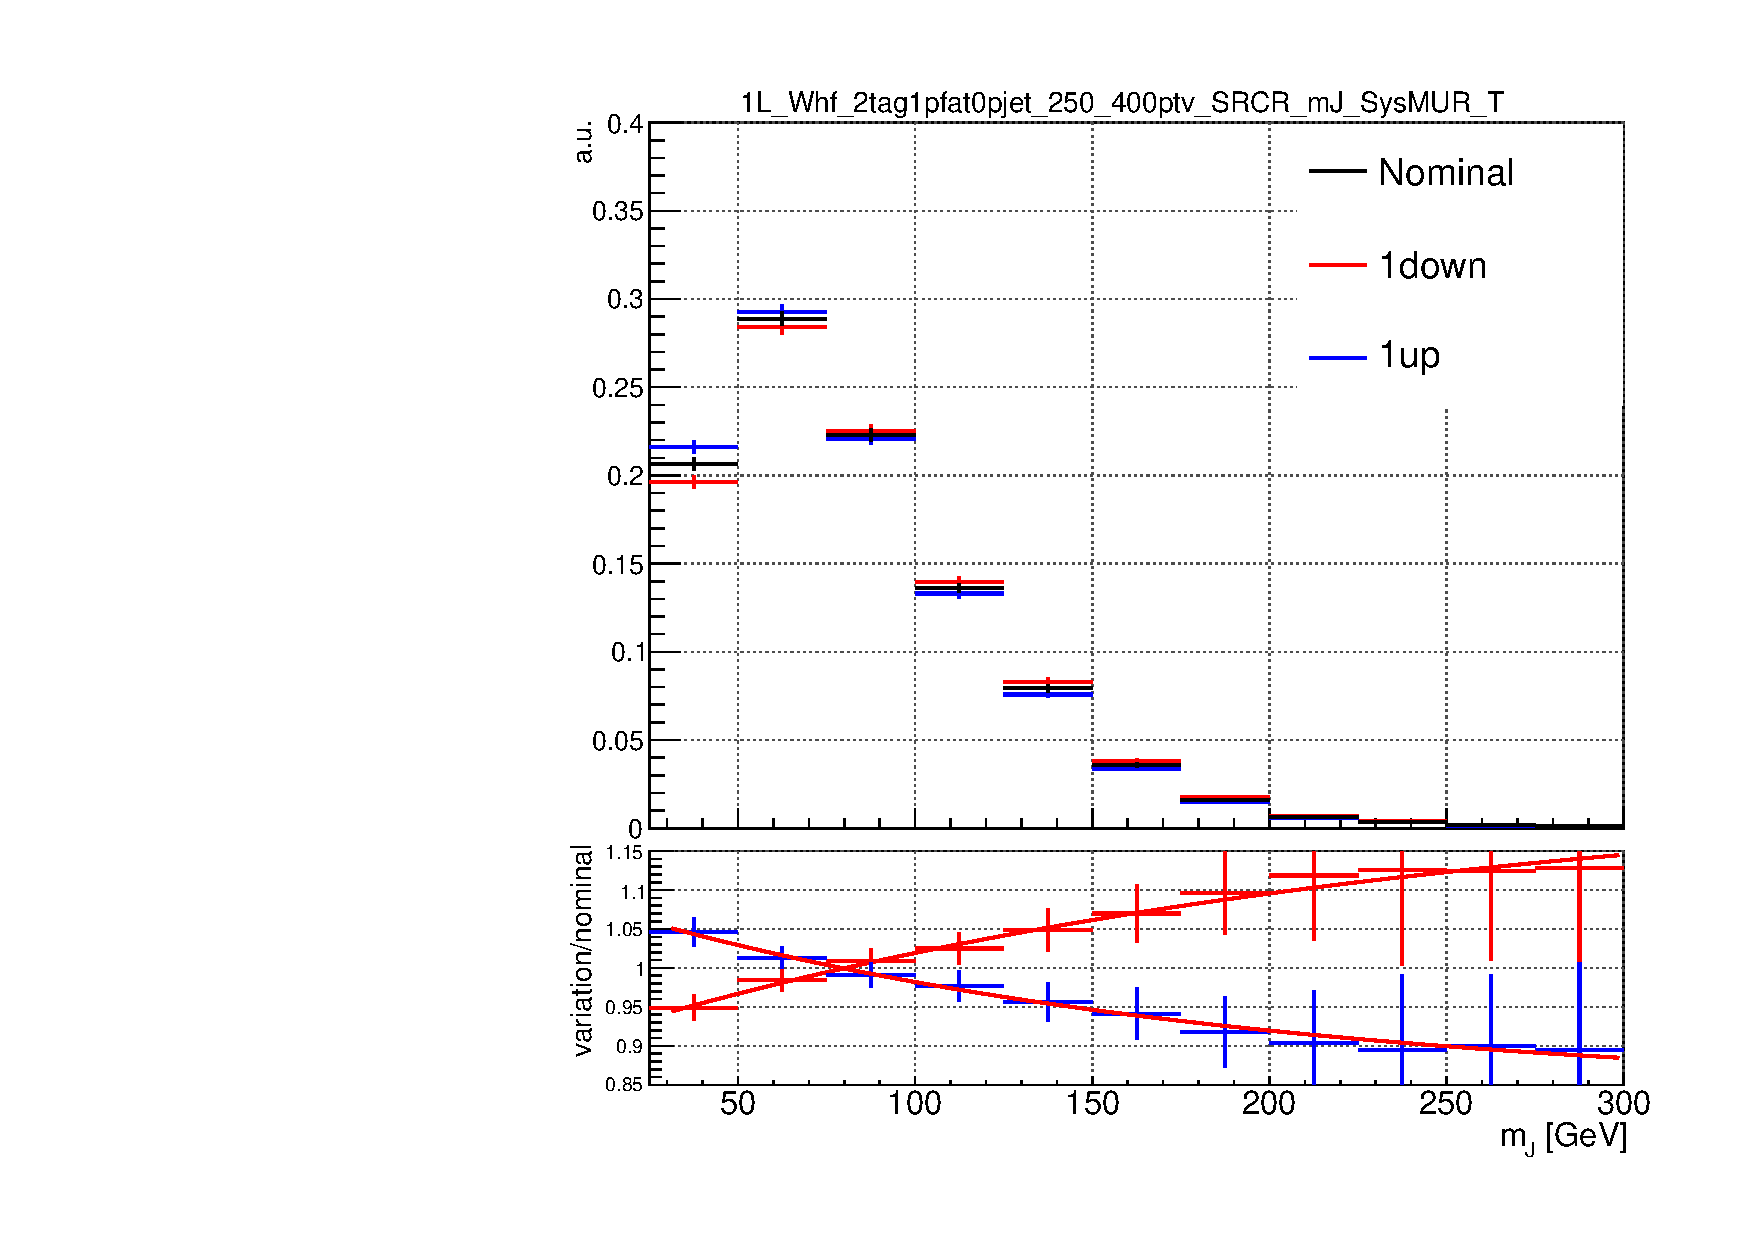
\includegraphics[width=\textwidth]{chapters/6.vhbb_boosted/figs/1L_Whf_2tag1pfat0pjet_250_400ptv_SRCR_mJ_SysMUR_T_Norm.pdf}
      \caption{}
      \label{fig:vhbb muR shape fitted sub1}
    \end{subfigure}%
    \begin{subfigure}{.4\textwidth}
      \centering
      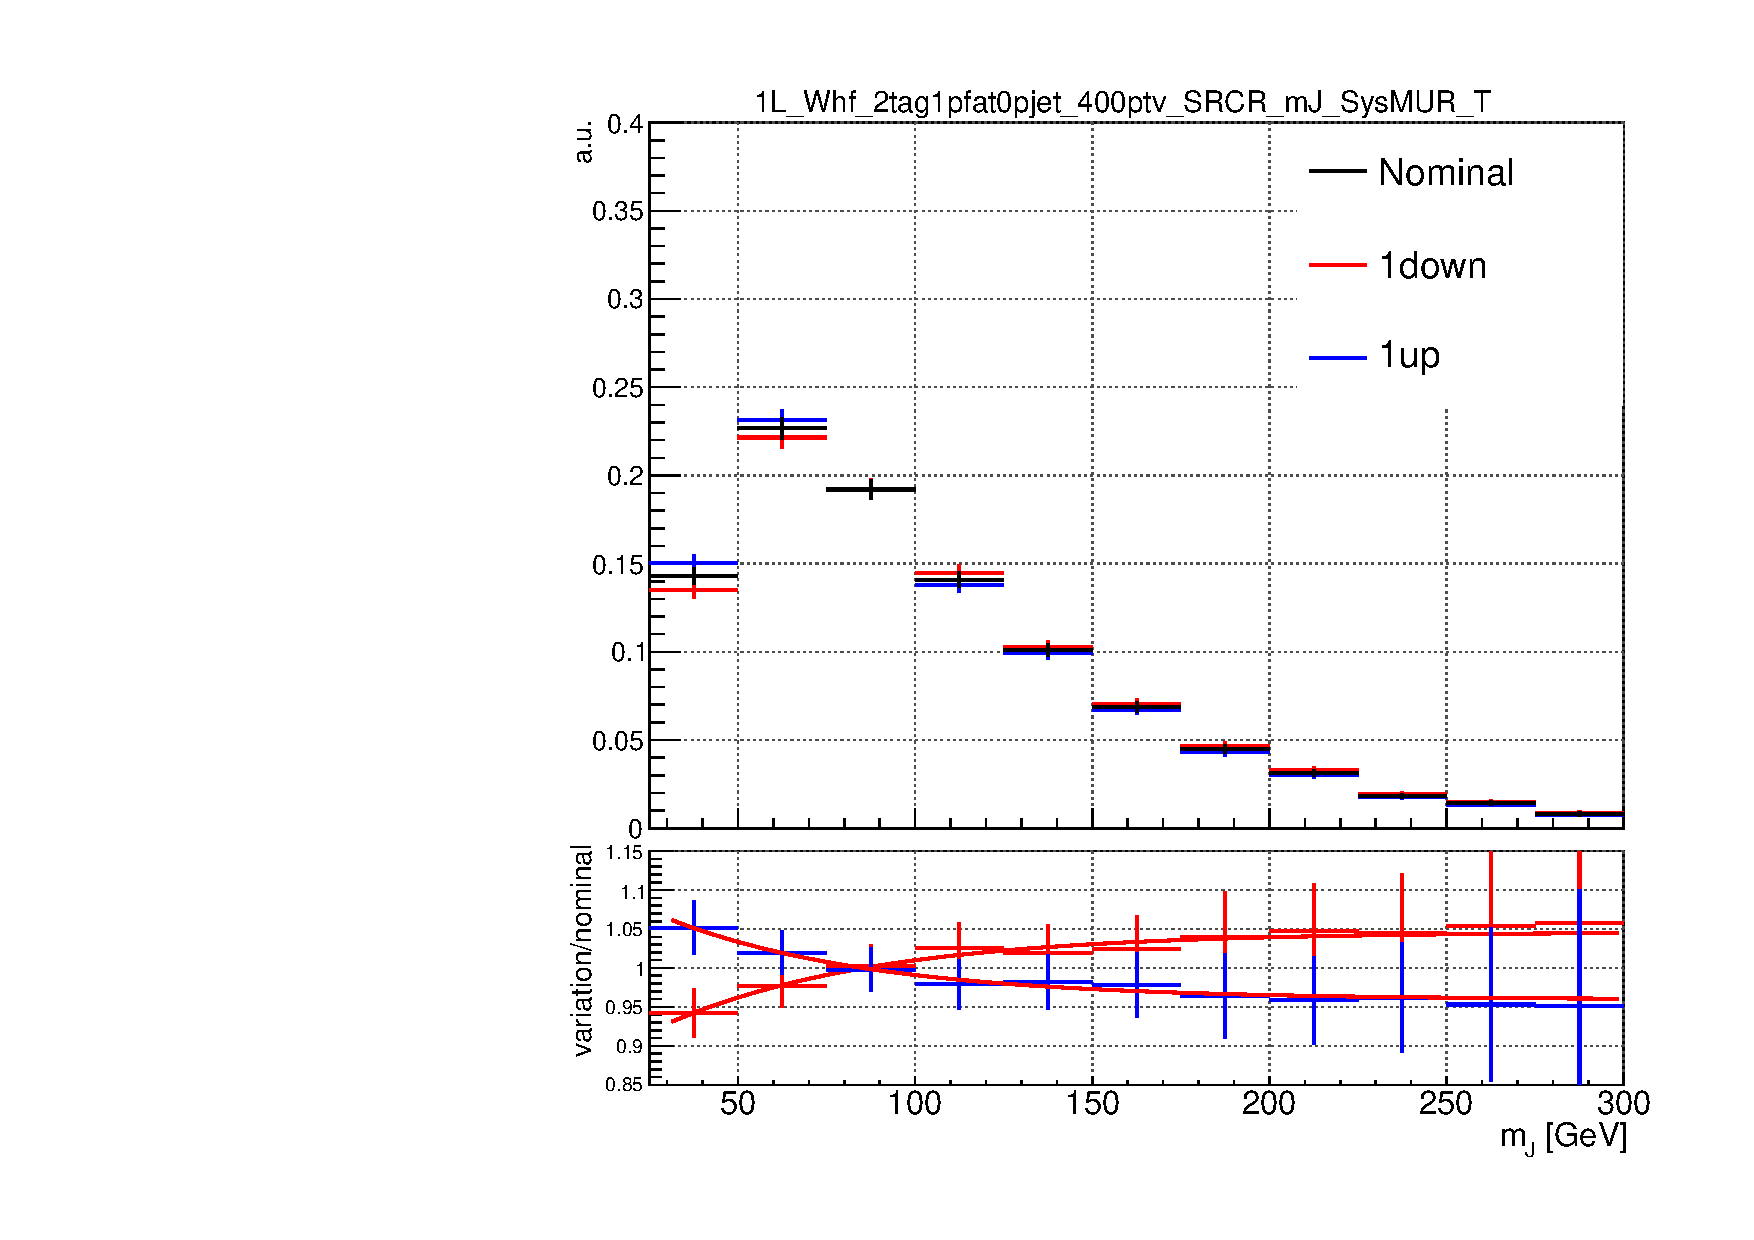
\includegraphics[width=\textwidth]{chapters/6.vhbb_boosted/figs/1L_Whf_2tag1pfat0pjet_400ptv_SRCR_mJ_SysMUR_T_Norm.pdf}
      \caption{}
      \label{fig:vhbb muR shape fitted sub2}
    \end{subfigure}
    \vspace{-0.5em}
    \caption{Normalised distributions of leading fat jet mass $m_J$ for medium (\ref{fig:vhbb muR shape fitted sub1}) and high (\ref{fig:vhbb muR shape fitted sub2}) \pTV analysis regions for W+heavy-flavour-jets in the 0 lepton channel.
    Merged in heavy flavours, high and low purity signal regions.
    The renormalisation scale $\mu_R$ has been varied by a factor of 2 (``1up'') and 0.5 (``1down''). An exponential function has been fit to the ratio.}
    \label{fig:vhbb muR shape fitted}
\end{figure}

\subsubsection{Acceptance Uncertainties}
Several different types of acceptance uncertainties have been calculated. These are implemented as nuisance parameters in the fit and for the most part account for the migration of events between different analysis regions. The list acceptance uncertainties relevant to the V+jets processes are given summarised below.
%
\begin{itemize}
    \item \textbf{Overall normalisation:} only relevant where normalisation cannot be left floating (i.e. determined in the fit).
    %
    \item \textbf{SR-to-CR relative acceptance:} the uncertainty on the normalisation of the signal region due to events migrating between the signal and control regions.
    %
    \item \textbf{HP-to-LP relative acceptance:} the uncertainty on the normalisation of the high-purity (HP) signal region due to events migrating between the high- and low-purity signal regions.
    %
    \item \textbf{Medium-to-high} \pTV \textbf{relative acceptance:} describes any 'shape' effect in \pTV distribution, given that the analysis only uses two \pTV bins (medium and high).
    %
    \item \textbf{Flavour relative acceptance:} for each flavour V$xx$, where $xx\in$ \{bc,bl,cc\} the ratio of V$xx$/Vbb events is calculated. This corresponds to the uncertainty of Vbb events due to the miss-tagging of other flavours V$xx$. 
\end{itemize}
%
The uncertainties on different systematics are summed in quadrature to give a total uncertainty on each region. A summary of the different acceptance uncertainties that were derived in this way and subsequently applied in the fit are given in \cref{tab:Vjets acceptance uncerts}. An effort has been made, wherever possible, to harmonise similar uncertainties across different analysis regions and channels.


\subsection{Vector Boson + Jets Modelling}
The background processes involving $W$ or $Z$ boson decays into leptons (including those in which the $W$ boson arises from a top-quark decay) are collectively referred to as electroweak (EW), or V+jets, backgrounds. \Wjets events are most relevant to the 1-lepton channel via the leptonic decay of W$\rightarrow \ell\nu$. In the event of W$\rightarrow \tau\nu$, and subsequent decay of the $\tau$, or the lack of the successful reconstruction of the $e$ or $\mu$, \Wjets can also contribute to the 0-lepton channel. Meanwhile, Z+jets contributes primarily to the 0- and 2-lepton channels via the processes Z$\rightarrow \nu\nu$ and Z$\rightarrow \ell\ell$ respectively.

Modelling is used to predict the outcomes of the analysis and to assess the impact of sources of different systematic uncertainty. Signal and background modelling has has primarily consisted of using Monte Carlo (MC) generators to produce simulated events. The uncertainties on the simulated output must be well understood to perform a successful analysis. To achieve this, a set of ``nominal'' samples are first defined as a reference to which different variations can be compared. The nominal samples are chosen as the best possible representation of the underlying physical process. ``Alternative'' samples are used to understand the systematic uncertainties on the nominal samples. To generate an alternative sample, some aspect of the model is varied, and the simulation is re-run. A comparison back to the nominal sample gives a handle on the systematic uncertainty associated with the model parameter which was changed. Detailed information can be found in \cite{Bell:2316951}. In order to access uncertainties associated with the use of MC generators, variations of the data are produced using alternative generators or variation of nominal generator parameters. The variation of nominal generator parameters can in certain cases be implemented using internal weight variations stored alongside the nominal events, and in other cases a new independent sample must be generated. The nominal generator used for V+jets events is \textsc{Sherpa 2.2.1}, while \textsc{MadGraph5\_aMC@NLO+Pythia8} (which uses different parton showering models) is used as an alternative generator. As production of large MC samples is computationally expensive, a feature of state of the art simulation packages is to store some sources of variation as internal event weights, which can be generated alongside the nominal samples, saving computation time. Several sources of uncertainty, summarised in \cref{tab:sources of uncertainty}, have been assessed.

%
\begin{table}[!htbp] 
  \footnotesize\centering
  \setlength{\tabcolsep}{0.5em} % for the horizontal padding
  %\def\arraystretch{1.4} 
  \begin{tabular}{l|c|c|c|c}
      \toprule\hline
      \multicolumn{5}{c}{V+jets Acceptance Uncertainties}            
      \\ \hline
      \textbf{Boson}      & \multicolumn{2}{c|}{\textbf{W}} & \multicolumn{2}{c}{\textbf{Z}} 
      \\ \hline
      \textbf{Channel}    & 0L          & 1L         & 0L         & 2L          
      %\\ \hline
      %Vbb Norm.           &   30\%      &     -      &     -      &          -  
      \\ \hline
      SR-to-CR               &   90\%$^\dagger$         & 40\%$^\dagger$ &      40\%     & -         
      \\ \hline
      HP-to-LP SR               & \multicolumn{2}{c|}{18\%}             &   18\%      & -         
      \\ \hline
      Medium-to-high $p_T^V$ &   30\%      & 10\%$^*$       & \multicolumn{2}{c}{10\%}          
      \\ \hline
      Channel relative acceptance             &   20\%      &   -        &    16\%    & -
      \\ \hline
      Vbc/Vbb             & \multicolumn{4}{c}{30\%}                       
      \\ \hline
      Vbl/Vbb             & \multicolumn{4}{c}{30\%}                       
      \\ \hline
      Vcc/Vbb             & \multicolumn{4}{c}{20\%}                       
      \\ \hline
      Vcl Norm.           & \multicolumn{4}{c}{30\%}                       
      \\ \hline
      Vl Norm.            & \multicolumn{4}{c}{30\%}                       
      \\ \hline\bottomrule
  \end{tabular}
  \caption{
    \Vjets acceptance uncertainties \cite{Dao:2688371}.
    \Wjets SR and CR uncertainties marked with a superscript $\dagger$ are correlated.
    The 1L \Wjets medium-to-high \pTV uncertainty marked by $*$ is applied as independent and uncorrelated NPs in both HP and LP signal regions.
    %The 0L \Wjets Wbb Norm uncertainty is only applied when a floating normalisation for Wbb cannot be obtained from the 1L channel.
    %A 30\% uncertainty for \Zbb norm is applied in the 1L channel when a floating normalisation for \Zbb cannot be obtained from the 0L or 2L channels.
  }
  \label{tab:Vjets acceptance uncerts}
\end{table}
%

\subsection{Diboson Modelling}



\section{Results}\label{sec:vhbb_results}

\begin{comment}
  paper abstract
  The measured
  signal strength, defined as the ratio of the measured signal yield to
  that predicted by the Standard Model, is $0.72 ^{+0.39}_{-0.36}$
  corresponding to an observed (expected) significance of 2.1 (2.7)
  standard deviations. Cross-sections of associated production of a
  Higgs boson decaying into $b$ quark pairs with a $W$ or $Z$ gauge
  boson, decaying into leptons, are measured in two exclusive
  vector boson transverse momentum regions, 250--\SI{400}{\GeV} and above \SI{400}{\GeV}, and
  interpreted as constraints on anomalous couplings in the framework of
  a Standard Model effective field theory.

  %For a Higgs boson mass of \SI{125}{\GeV}, an excess of events over the expected background from other Standard Model processes is found
  %with an observed significance of $3.5$ standard deviations, compared to an expectation of $3.0$
  %standard deviations. This excess provides evidence for the Higgs boson decay into b-quarks
  %and for its production in association with a vector boson. Assuming the Standard Model production 0.19
  %cross-section, the results are consistent with the value of the Yukawa coupling to b-quarks in the Standard Model.
\end{comment}



\subsection{Fit Model}

A global profile likelihood fit is used to extract the signal strength $\mu$ and its significance from the data. This statistical setup treats each bin as a Poisson counting experiment. The combined likelihood over $N$ bins, without considering sources of systematic uncertainty, is given by
%
\begin{equation}
    \mathcal{L}(\mu) = \prod_{i=1}^N \frac{(\mu s_i + b_i)^{n_i}}{n_i!} \exp \left[ - (\mu s_i + b_i) \right],
\end{equation}
%
where $s_i$ ($b_i$) is the expected number of signal (background) events in bin $i$, and $n_i$ is the number of events observed in data in bin $i$. The presence of systematic uncertainties which can affect the expected numbers of signal and background events necessitates the addition of nuisance parameters (NPs), $\theta$, to the likelihood. Each source of systematic uncertainty for V+jets samples discussed in the previous section was implemented as a NP $\theta_j$ in the fit. The presence of NPs modifies the likelihood as 
%
\begin{equation}
    \mathcal{L}(\mu) \rightarrow \mathcal{L}(\mu, \theta) = \mathcal{L}(\mu) \times \mathcal{L}(\theta) , \quad s_i \rightarrow s_i(\theta) , \quad b_i \rightarrow b_i(\theta),
\end{equation}
%
where
%
\begin{equation}
    \mathcal{L}(\theta) = \prod_{\theta_j \in \theta} \frac{\exp\left[{-\theta_j^2/2}\right]}{\sqrt{2\pi}}.
\end{equation}
%


\subsection{Post-fit Results}

Post-fit $m_J$ distributions in the high-purity medium \pTV regions for the 0- and 2-lepton channels are shown in \cref{fig:vhbb postfit plots}. The plots show large falling backgrounds, predominantly made up of \Wjets and Z+jets events, and a signal distribution corresponding to the Standard Model Higgs boson peaking around $m_H = 125$ GeV.

\begin{figure}[!htbp]
  \centering
  \begin{subfigure}{.4\textwidth}
    \centering
    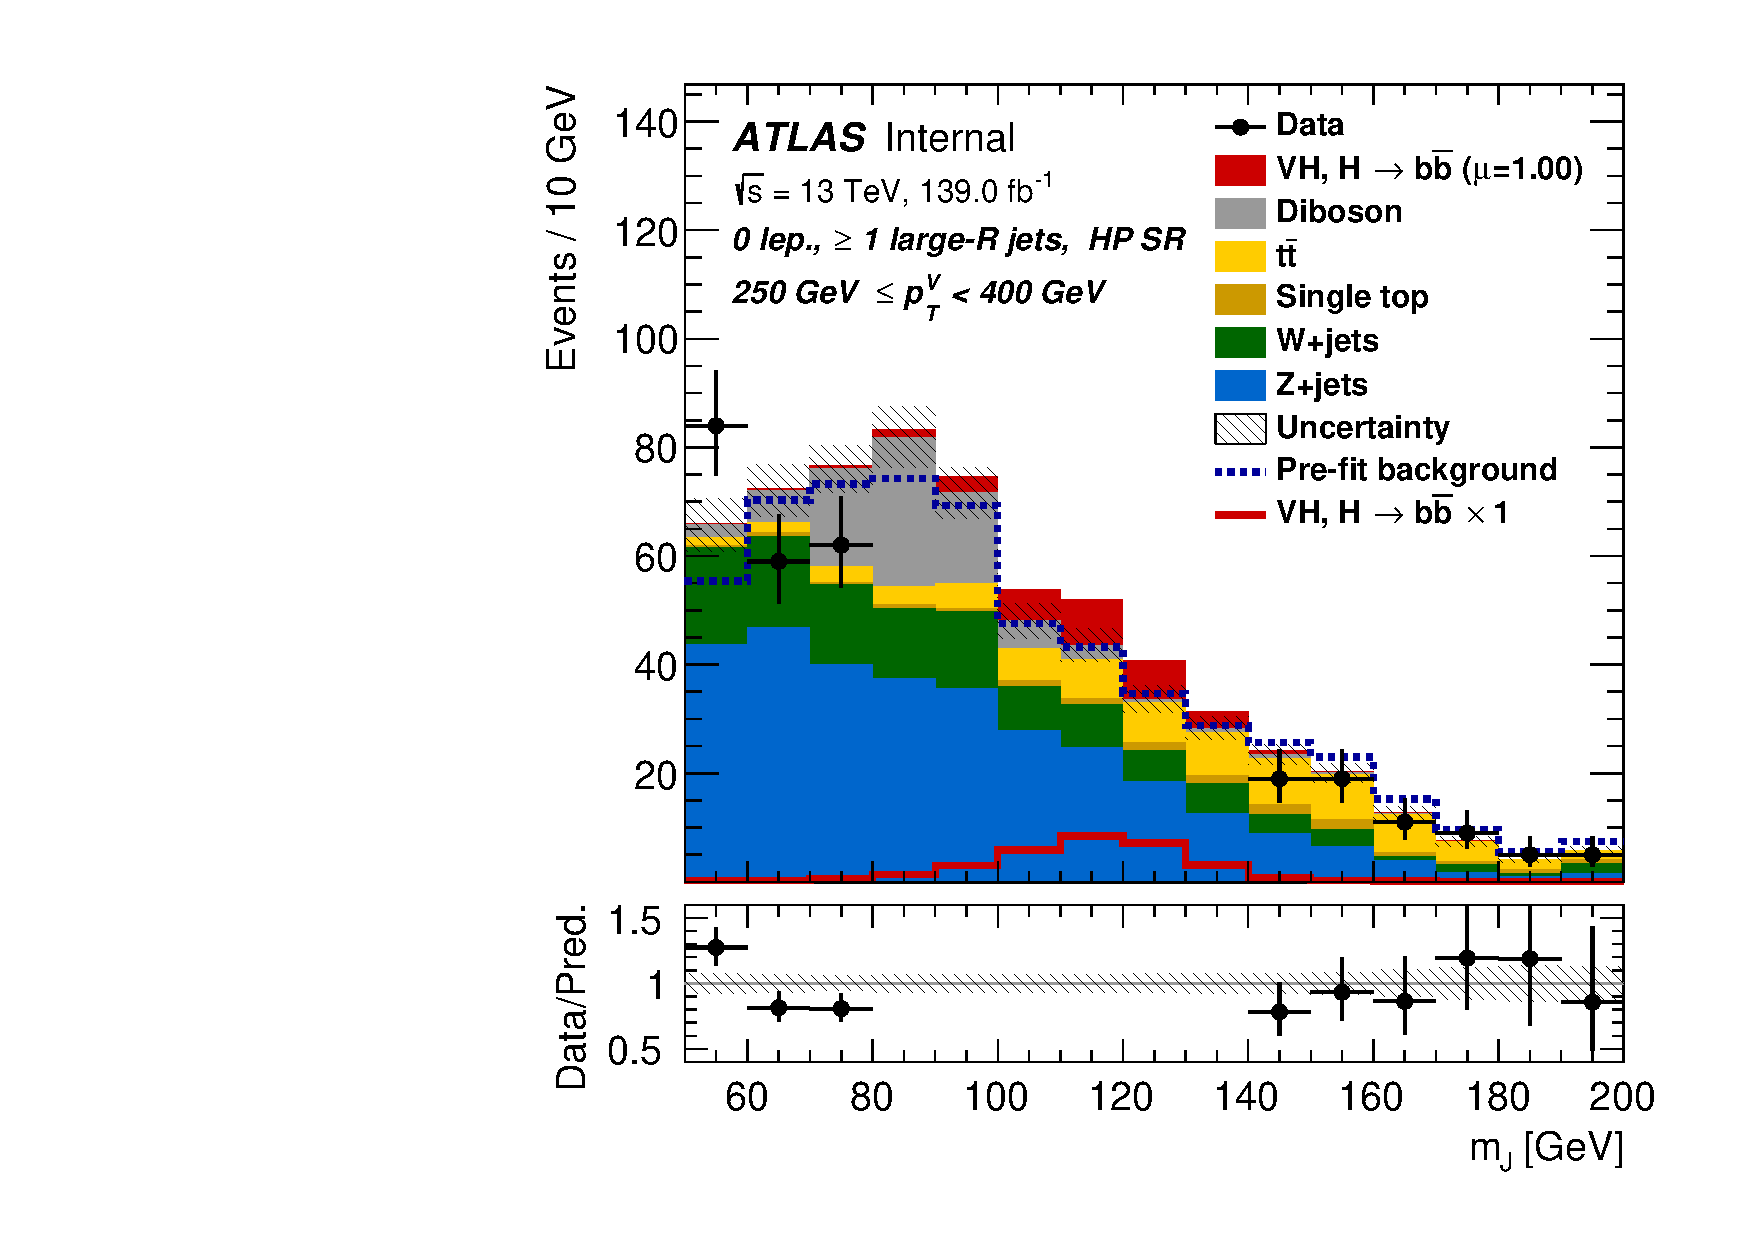
\includegraphics[width=\textwidth]{chapters/6.vhbb_boosted/figs/Region_BMax400_BMin250_incFat1_Fat1_Y6051_DSRnoaddbjetsr_T2_L0_distmBB_J0_GlobalFit_conditionnal_mu1.pdf}
  \end{subfigure}%
  \begin{subfigure}{.4\textwidth}
    \centering
    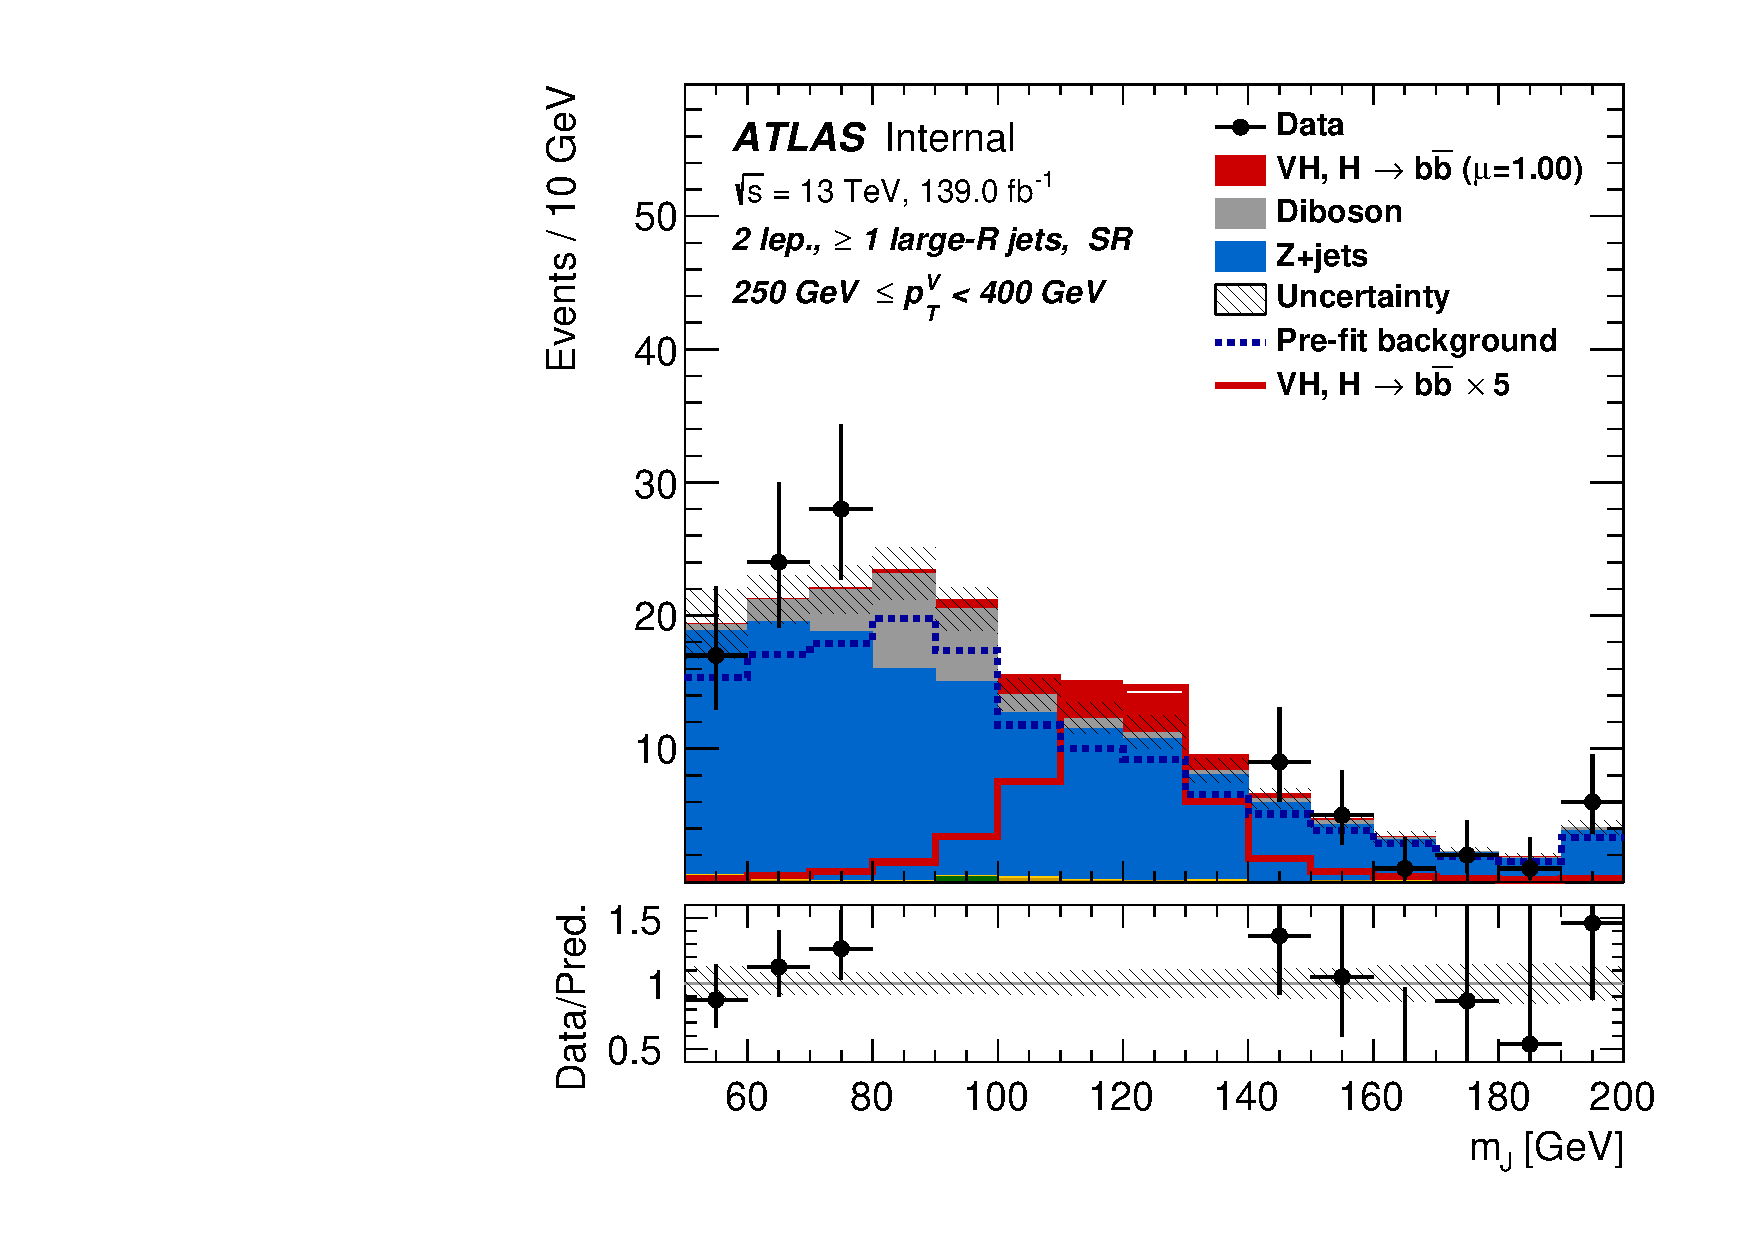
\includegraphics[width=\textwidth]{chapters/6.vhbb_boosted/figs/Region_distmBB_J0_L2_T2_DSR_Y6051_incJet1_Fat1_incFat1_BMin250_BMax400_GlobalFit_conditionnal_mu1.pdf}
  \end{subfigure}
  \caption{
    Post-fit distributions for the 0-lepton (left) and 2-lepton (right) channels in the high purity medium \pTV region, obtained in the combined conditional $\mu=1$ fit to data. The last bin of each plot is an overflow bin.
  }
  \label{fig:vhbb postfit plots}
\end{figure}


\begin{table}[tb]
    \begin{center}
    \begin{tabular}{ l | l  c c }
        \toprule
        \multicolumn{2}{l}{Source of uncertainty}  & Avg. impact \\
        \toprule
        \multicolumn{2}{l}{Total} & 0.372 \\
        \multicolumn{2}{l}{Statistical} & 0.283 \\
        %\multicolumn{2}{l}{$\hookrightarrow$ Data stat only} & 0.248 \\
        %\multicolumn{2}{l}{$\hookrightarrow$ Floating normalisations} & 0.094 \\
        \multicolumn{2}{l}{Systematic} & 0.240 \\
        \midrule
        \multicolumn{3}{l}{Experimental uncertainties}\\
        \midrule
        \multicolumn{2}{l}{\SmallR\  jets} &  0.038 \\
        \multicolumn{2}{l}{\LargeR\  jets} &  0.133 \\
        %\multicolumn{2}{l}{$E_{T}^{\textrm{miss}}$} & 0.007 \\
        \multicolumn{2}{l}{\met} & 0.007 \\
        \multicolumn{2}{l}{Leptons} & 0.010 \\
        \multirow{3}{*}{$b$-tagging~~~} & $b$-jets & 0.016 \\
        & $c$-jets &  0.011 \\
        & light-flavour jets & 0.008 \\
        & extrapolation & 0.004 \\
        \multicolumn{2}{l}{Pile-up} & 0.001 \\
        \multicolumn{2}{l}{Luminosity} & 0.013 \\
        \midrule
        \multicolumn{3}{l}{Theoretical and modelling uncertainties}\\
        \midrule
        \multicolumn{2}{l}{Signal} & 0.038 \\
        %\multicolumn{3}{l}{} \\
        \multicolumn{2}{l}{Backgrounds} & 0.100 \\
        \multicolumn{2}{l}{$\hookrightarrow$ $Z$~+~jets} & 0.048 \\
        \multicolumn{2}{l}{$\hookrightarrow$ $W$~+~jets} & 0.058 \\
        \multicolumn{2}{l}{$\hookrightarrow$ $t\bar{t}$} & 0.035 \\
        \multicolumn{2}{l}{$\hookrightarrow$ Single top quark} & 0.027 \\
        \multicolumn{2}{l}{$\hookrightarrow$ Diboson} & 0.032 \\
        \multicolumn{2}{l}{$\hookrightarrow$ Multijet} & 0.009 \\
        \midrule
        \multicolumn{2}{l}{MC statistical} & 0.092 \\
        \bottomrule
    \end{tabular}
    \end{center}
    \caption{
        Breakdown of the absolute contributions to the uncertainty in $\mu_{VH}^{bb}$ inclusive in \pTV. 
        The sum in quadrature of the systematic uncertainties attached to the categories differs from the total systematic uncertainty due to correlations. 
        The reported values represent the average between the positive and negative uncertainties on $\mu_{VH}^{bb}$.
        %Average impact refers to the mean of the systematic uncertainty up and down variations. 
    }
    \label{tab:mu_syst_unc}
\end{table}
    


\section{Conclusion}

Work has been carried out as part of the boosted VHbb analysis group to understand, and implement in the global profile likelihood fit, systematic uncertainties on V+jets samples. This background modelling work is an essential part of the success of the analysis. So far the fit has proved stable with the inclusion of the V+jets uncertainties, and detailed studies are now underway to determine the causes behind any observed pulls of the added NPs. Additional work is ongoing to help with the derivation of uncertainties on diboson samples, another important background. The analysis is already advanced, and is now progressing into its final stages. Publication is expected in the new year.

This analysis would benefit greatly from the improved high \pt \btagging enabled by \GNN.
